\documentclass[tikz,border=10pt]{standalone}
\usepackage{ctex}
\usetikzlibrary{positioning, calc}

\begin{document}
本小测配合该图食用
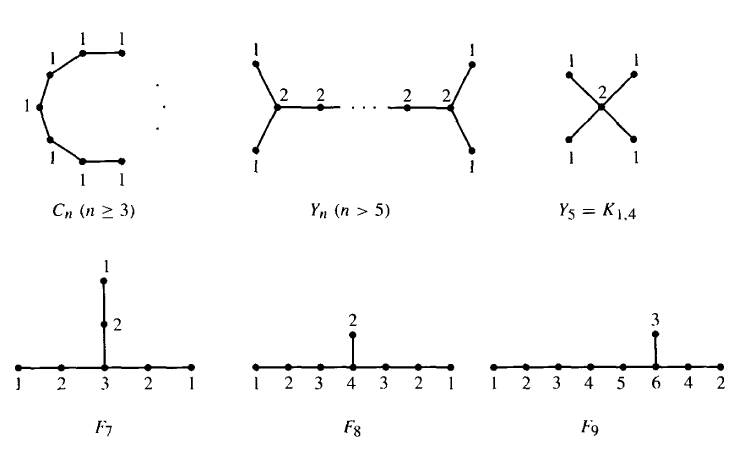
\includegraphics[width=\textwidth]{photo/tikz小测.jpg}
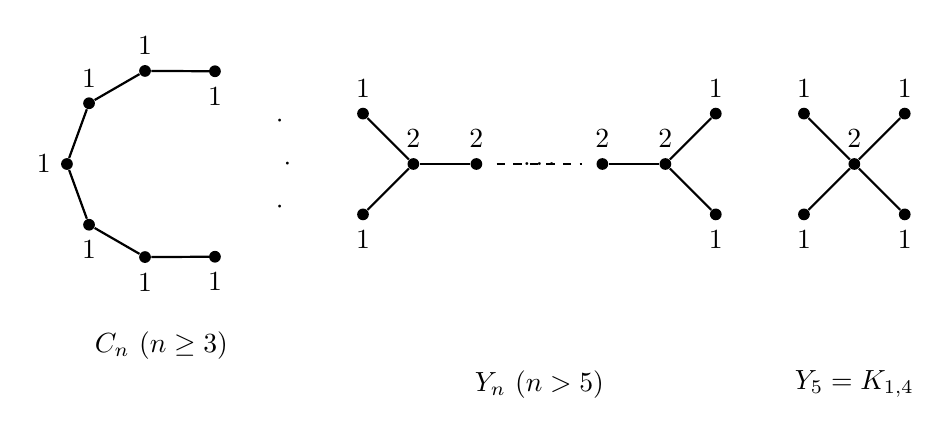
\begin{tikzpicture}[
    scale=0.8,
    dot/.style={fill=black, circle, inner sep=1.5pt},
    edge/.style={thick},
    lbl/.style={font=\footnotesize}
]

%% ---------------------------------------------------------
%% 第一行
%% ---------------------------------------------------------

% --- 图 Cn (n >= 3) ---
\begin{scope}[shift={(0,0)}]
    % 定义节点位置 (模拟 C 形)
    \coordinate (c1) at (60:1.7);
    \coordinate (c2) at (100:1.5);
    \coordinate (c3) at (140:1.5);
    \coordinate (c4) at (220:1.5);
    \coordinate (c5) at (260:1.5);
    \coordinate (c6) at (300:1.7);

    % 绘制点和标签 (权重全是 1)
    \node[dot,label=below:1] (n1) at (c1) {};
    \node[dot, label=above:1] (n1) at (c2) {};
    \node[dot, label=above:1] (n2) at (c3) {};
    \node[dot, label=left:1]  (n3) at (180:1.5) {};
    \node[dot, label=below:1] (n4) at (c4) {};
    \node[dot, label=below:1] (n5) at (c5) {};
    \node[dot,label=below:1] (n6) at (c6) {};
    
    % 绘制连线
    \draw[edge] (c1) -- (n1) -- (n2) -- (n3) -- (n4) -- (n5) -- (c6);
    
    % 绘制省略号
    \node at (0:2) {$\cdot$};
    \node at (20:2){$\cdot$};
    \node at (340:2){$\cdot$};
    % 标题
    \node[below=2cm] at (0,0) {$C_n \ (n \ge 3)$};
\end{scope}

% --- 图 Yn (n > 5) ---
\begin{scope}[shift={(6,0)}]
    % 左分叉
    \coordinate (L_center) at (-2,0);
    \node[dot, label=above:2] (L_c) at (L_center) {};
    \node[dot, label=above:1] (L_u) at ($ (L_center) + (-0.8, 0.8) $) {};
    \node[dot, label=below:1] (L_d) at ($ (L_center) + (-0.8, -0.8) $) {};
    \draw[edge] (L_u) -- (L_c) -- (L_d);
    
    % 右分叉
    \coordinate (R_center) at (2,0);
    \node[dot, label=above:2] (R_c) at (R_center) {};
    \node[dot, label=above:1] (R_u) at ($ (R_center) + (0.8, 0.8) $) {};
    \node[dot, label=below:1] (R_d) at ($ (R_center) + (0.8, -0.8) $) {};
    \draw[edge] (R_u) -- (R_c) -- (R_d);
    
    % 中间连接部分
    \coordinate (L_mid) at (-1,0);
    \coordinate (R_mid) at (1,0);
    \node[dot, label=above:2] (L_m) at (L_mid) {};
    \node[dot, label=above:2] (R_m) at (R_mid) {};
    
    \draw[edge] (L_c) -- (L_m);
    \draw[edge] (R_c) -- (R_m);
    \draw[edge, dashed, shorten >=5pt, shorten <=5pt] (L_m) -- (R_m); % 虚线或省略号区域
    \path (L_m) -- node {$\dots$} (R_m);
    
    % 标题
    \node[below=2.5cm] at (0,0) {$Y_n \ (n > 5)$};
\end{scope}

% --- 图 Y5 = K1,4 ---
\begin{scope}[shift={(11,0)}]
    \node[dot, label=above:2] (center) at (0,0) {};
    
    \node[dot, label=above:1] (tl) at (-0.8, 0.8) {};
    \node[dot, label=above:1] (tr) at (0.8, 0.8) {};
    \node[dot, label=below:1] (bl) at (-0.8, -0.8) {};
    \node[dot, label=below:1] (br) at (0.8, -0.8) {};
    
    \draw[edge] (tl) -- (center) -- (tr);
    \draw[edge] (bl) -- (center) -- (br);
    
    % 标题
    \node[below=2.5cm] at (0,0) {$Y_5 = K_{1,4}$};
\end{scope}

\end{tikzpicture}
%% ---------------------------------------------------------
%% 第二行
%% ---------------------------------------------------------
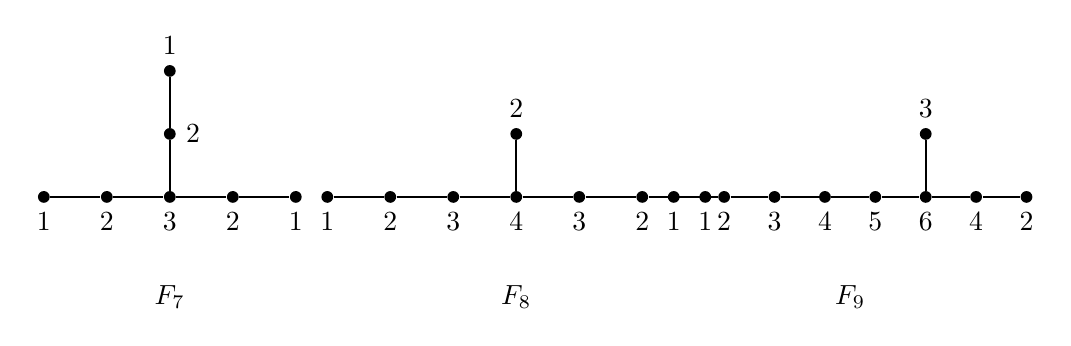
\begin{tikzpicture}[
    scale=0.8,
    dot/.style={fill=black, circle, inner sep=1.5pt},
    edge/.style={thick},
    lbl/.style={font=\footnotesize}
]
% --- 图 F7 ---
\begin{scope}[shift={(0,-5)}]
    % 水平点: 1, 2, 3, 2, 1
    \foreach \x/\w in {-2/1, -1/2, 0/3, 1/2, 2/1} {
        \node[dot, label=below:\w] (h\x) at (\x, 0) {};
    }
    % 连线
    \draw[edge] (h-2) -- (h-1) -- (h0) -- (h1) -- (h2);
    
    % 垂直点: 2, 1 (在3之上)
    \node[dot, label=right:2] (v1) at (0, 1) {};
    \node[dot, label=above:1] (v2) at (0, 2) {};
    
    \draw[edge] (h0) -- (v1) -- (v2);
    
    % 标题
    \node[below=1cm] at (0,0) {$F_7$};
\end{scope}

% --- 图 F8 ---
\begin{scope}[shift={(5.5,-5)}]
    % 水平点: 1, 2, 3, 4, 3, 2, 1
    \foreach \x/\w in {-3/1, -2/2, -1/3, 0/4, 1/3, 2/2, 3/1} {
        \node[dot, label=below:\w] (h\x) at (\x, 0) {};
    }
    % 连线
    \draw[edge] (h-3) -- (h-2) -- (h-1) -- (h0) -- (h1) -- (h2) -- (h3);
    
    % 垂直点: 2 (在4之上)
    \node[dot, label=above:2] (v1) at (0, 1) {};
    
    \draw[edge] (h0) -- (v1);
    
    % 标题
    \node[below=1cm] at (0,0) {$F_8$};
\end{scope}

% --- 图 F9 ---
\begin{scope}[shift={(12,-5)}]
    % 水平点: 1, 2, 3, 4, 5, 6, 4, 2
    % 注意：为了对齐，我们把标号为6的点设为中心 (0,0)
    % 序列: 1(x=-5), 2(-4), 3(-3), 4(-2), 5(-1), 6(0), 4(1), 2(2)
    
    \foreach \x/\w in {-5/1, -4/2, -3/3, -2/4, -1/5, 0/6, 1/4, 2/2} {
        \node[dot, label=below:\w] (h\x) at (\x*0.8, 0) {}; % 稍微缩紧间距 *0.8
    }
    
    % 连线
    \draw[edge] (h-5) -- (h-4) -- (h-3) -- (h-2) -- (h-1) -- (h0) -- (h1) -- (h2);
    
    % 垂直点: 3 (在6之上)
    \node[dot, label=above:3] (v1) at (0, 1) {};
    
    \draw[edge] (h0) -- (v1);
    
    % 标题 (根据中心点偏移调整)
    \node[below=1cm] at (-1.2,0) {$F_9$};
\end{scope}

\end{tikzpicture}
\end{document}